\chapter{Der Slow-Koinzidenzkreis}
\section{Theoretische Grundlagen}
\subsection{Szintillationsspektrometer}

Zur Detektion der $\gamma$-Strahlung werden Szintillationsspektrometer eingesetzt. 
Diese bestehen aus einem NaI(Tl)-Szintillationskristall, einem Photomultiplier (PMT) sowie einer elektronischen Ausleseeinheit mit integriertem Vorverstärker.

Trifft ionisierende Strahlung auf den Szintillationskristall, wird ein Teil der deponierten Energie in Form von Lichtblitzen im sichtbaren Spektralbereich emittiert. 
Diese Photonen treffen auf die Photokathode des Photomultipliers und lösen dort durch den Photoeffekt Elektronen aus. 
Durch die anschließende Vervielfachung der Elektronen an einer Reihe von Dynoden entsteht ein elektrischer Impuls, dessen Amplitude proportional zur im Kristall deponierten Energie ist.

Das Signal kann an verschiedenen Stellen des Photomultipliers abgegriffen werden. 
Für Zeitmessungen wird ein schneller Signalzweig genutzt, dessen Impulse an der Anode entnommen werden. 
Aufgrund ihrer kurzen Anstiegszeiten ermöglichen diese Signale eine hohe zeitliche Auflösung. 
Für die Energiemessung wird dagegen das Signal an einer der letzten Dynoden abgegriffen. 
Dieses besitzt eine bessere Amplitudenauflösung und eignet sich daher besonders zur Aufnahme und Auswertung von Energiespektren.

Das Szintillationsspektrometer erlaubt somit sowohl die präzise Bestimmung von Zeitdifferenzen als auch die Messung der Energie einfallender $\gamma$-Quanten.

\subsection{Die Zerfallsschemata von $^{22}$Na und $^{133}$Ba}

Zur Bestimmung der Lebensdauer des angeregten $\frac{5}{2}^{+}$-Zustands von $^{133}_{55}\mathrm{Cs}$ wird eine $^{133}_{56}\mathrm{Ba}$-Quelle verwendet. 
Beim Zerfall von $^{133}*{56}\mathrm{Ba}$ werden verschiedene angeregte Zustände des Tochterkerns besetzt. 
Besonders relevant ist dabei der Übergang, bei dem unter Aussendung eines $\gamma$-Quants der Energie 356,keV der $\frac{5}{2}^{+}$-Zustand von $^{133}_{55}\mathrm{Cs}$ erzeugt wird, da dieser ~ $2/3$ der Zeit stat findet (Abildung:\ref{fig:ZerfallBa}). 
Das zugehörige Signal dient als Startsignal der Lebensdauermessung.

Der angeregte Kernzustand zerfällt anschließend durch Emission eines weiteren $\gamma$-Quants mit einer Energie von 81,keV in den Grundzustand. 
Dieses Photon wird als Stoppsignal registriert. 
Die Zeitdifferenz zwischen beiden Ereignissen entspricht der Aufenthaltsdauer des Kerns im angeregten Zustand und ermöglicht somit die Bestimmung seiner mittleren Lebensdauer.

Neben dem beschriebenen Zerfallspfad existieren weitere Übergänge, über die der $\frac{5}{2}^{+}$-Zustand ebenfalls bevölkert werden kann. 
In diesen Fällen wird kein korrespondierendes 356-keV-Photon emittiert, sodass das später auftretende 81-keV-Photon keinem eindeutigen Startsignal zugeordnet werden kann. 
Werden zwei unabhängige Zerfallsereignisse zufällig innerhalb des Koinzidenzfensters registriert, entstehen sogenannte zufällige Koinzidenzen. 
Diese tragen zu einem Untergrund in der Zeitverteilung bei und können die Auswertung beeinflussen. 
Aufgrund der vergleichsweise geringen Aktivität der verwendeten Quelle ist ihr Beitrag jedoch klein.

Zur Kalibration des Messaufbaus wird zusätzlich eine $^{22}_{11}\mathrm{Na}$-Quelle eingesetzt. 
Dieses Nuklid zerfällt überwiegend durch $\beta^{+}$-Zerfall in $^{22}_{10}\mathrm{Ne}$ (Abbildung:\ref{fig:ZerfallNa})und emittiert dabei charakteristische $\gamma$-Strahlung mit einer Energie von 1274,5 keV.
Das entstandene Positron verliert seine kinetische Energie innerhalb kurzer Zeit in der umgebenden Materie und annihiliert anschließend mit einem Elektron. 
Dabei entstehen zwei Photonen mit jeweils 511,keV, die aufgrund der Impulserhaltung nahezu in entgegengesetzte Richtungen ausgesandt werden.

Da beide Annihilationsphotonen demselben Prozess entstammen, werden sie praktisch gleichzeitig erzeugt. 
Die Messung dieser Koinzidenzereignisse ermöglicht daher die Bestimmung der Zeitauflösung des Detektionssystems sowie die Kalibration der Zeitskala. 
Gleichzeitig eignet sich die Quelle aufgrund ihrer gut bekannten Photonenenergien für die Energiekalibration der verwendeten Detektoren.


\begin{figure}[htbp]
    \centering

    \begin{subfigure}{0.48\textwidth}
        \centering
        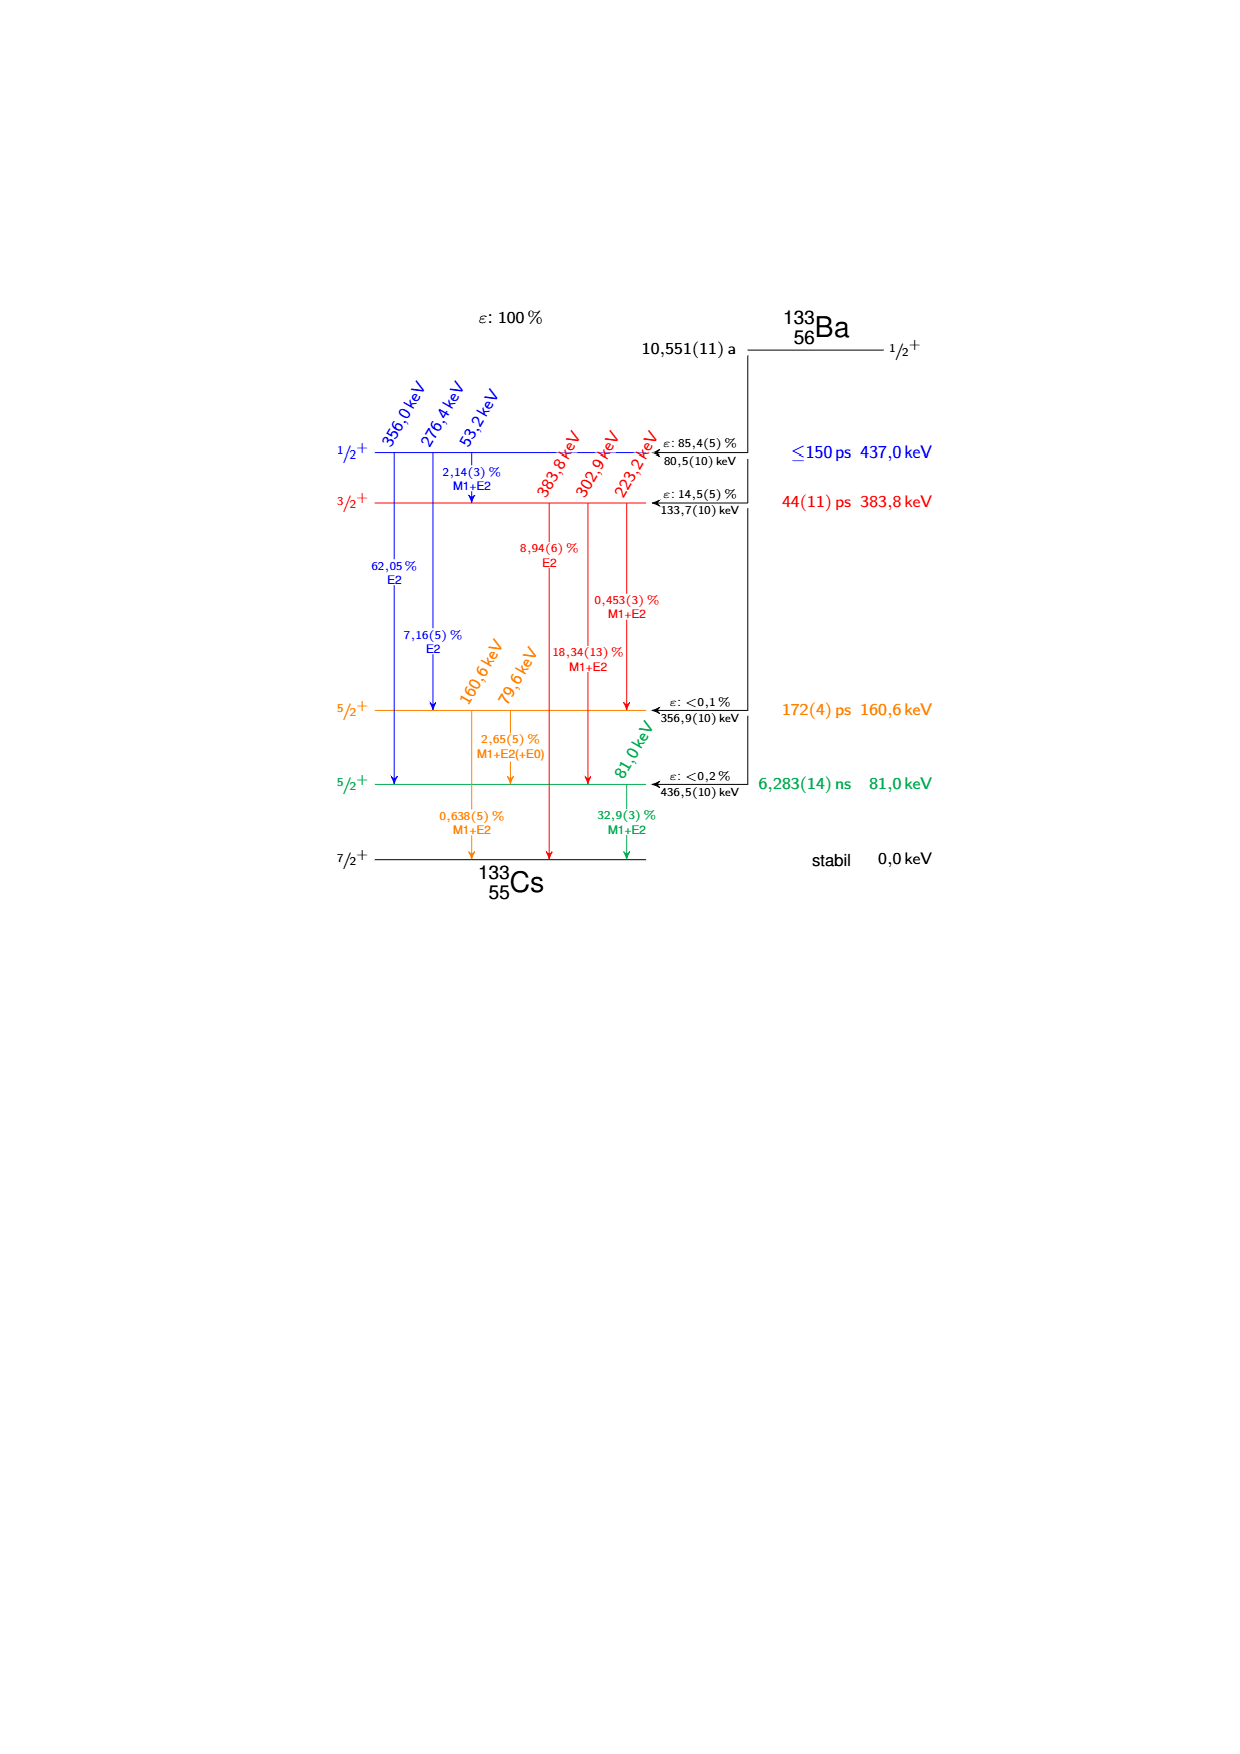
\includegraphics[width=\linewidth]{figs1/Ba.pdf}
        \caption{$^{133}$Ba}
        \label{fig:ZerfallBa}
    \end{subfigure}
    \hfill
    \begin{subfigure}{0.48\textwidth}
        \centering
        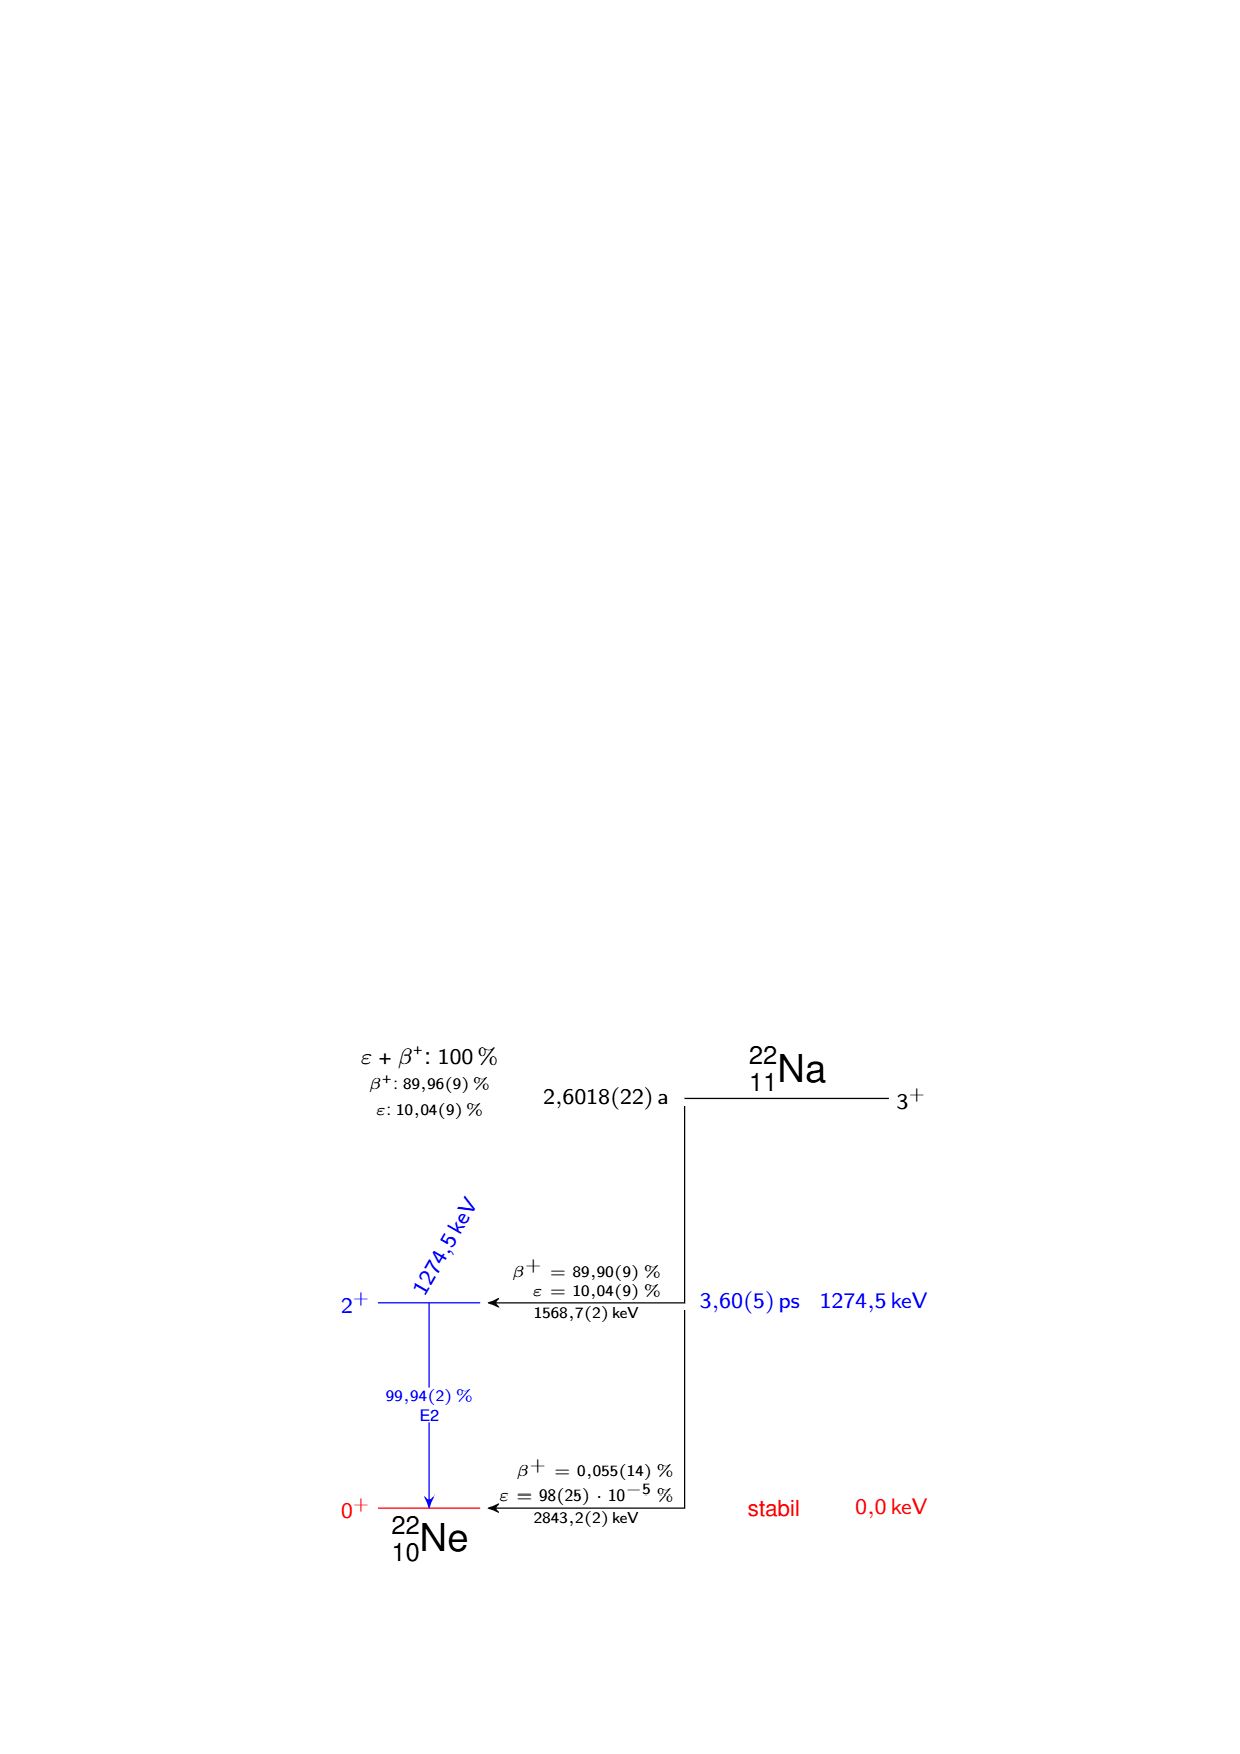
\includegraphics[width=\linewidth]{figs1/Na.pdf}
        \caption{$^{22}$Na}
        \label{fig:ZerfallNa}
    \end{subfigure}

    \caption{Zerfallsschemata der im Versuch verwendeten Isotope.}
    \label{fig:zerfallsschemata}
\end{figure}

\subsection{Slow und Fast}

%--------------------------------------------------------
\section{Einstellung des Slow-Koinzidenzkreises}
\subsection{Niedervolt-Versorgungsspannungen}
\subsection{Slow-Pulse des Photomultipliers}
\subsection{Triggerung mit dem SCA}
\section{Auswertung}
\subsection{Identifikation des Energiespektrum der Na-Quelle und Einstellung der Verstärkung}
\subsection{Aufnahme der Energiespektren der $^{22}$Na und $^{133}$Ba-Quellen}
\subsection{Einstellung des Einkanalfenster für die $^{22}$Na-Quelle}
\subsection{Herstellung der Slow-Koinzidenz}
\subsection{Energiekallibration des Slow-Koinzidenzkreises}
\subsection{$^{133}$Ba-Spektrum}
\subsection{Enrgieauflösung}
\subsection{Energieintervall des SCAs und Energien der CFD-Schwellen}
